\section{Systemarchitektur}\label{zitieren}

Wenn wir darüber sprechen, Hausarbeiten zu schreiben, dann brauchen wir in jedem
Fall eine gute Literaturverwaltung. \LaTeX~bietet uns hierfür mit BibTeX ein
sehr einfaches und verbreitetes Tool. Wir können es nutzen, um im Text zu
zitieren bzw. zu paraphrasieren und um uns dann ein Literaturverzeichnis
erstellen zu lassen. Genaugenommen arbeiten wir in diesem Template nicht mit
BibTeX, sondern mit BibLaTeX, welches einen besseren Umgang mit Umlauten und
Webseiten bietet. Ich verwende den Begriff BibTeX jedoch an dieser Stelle
weiter. \\ Damit das Arbeiten mit BibTeX möglich ist, brauchen wir unsere
Literatur als BibTeX Einträge in unserem Projekt. Ich habe hierfür ein
Verzeichnis (bibtex) angelegt, welches eine Datei (hauptdatei.bib) enthält. In
dieser Datei können wir unsere Literatureinträge hinterlegen. Glücklicherweise
bietet quasi jede Bibliotheksseite einen entsprechenden Export in BibTeX an: 
\FloatBarrier
\begin{figure}[ht!]
	\centering
	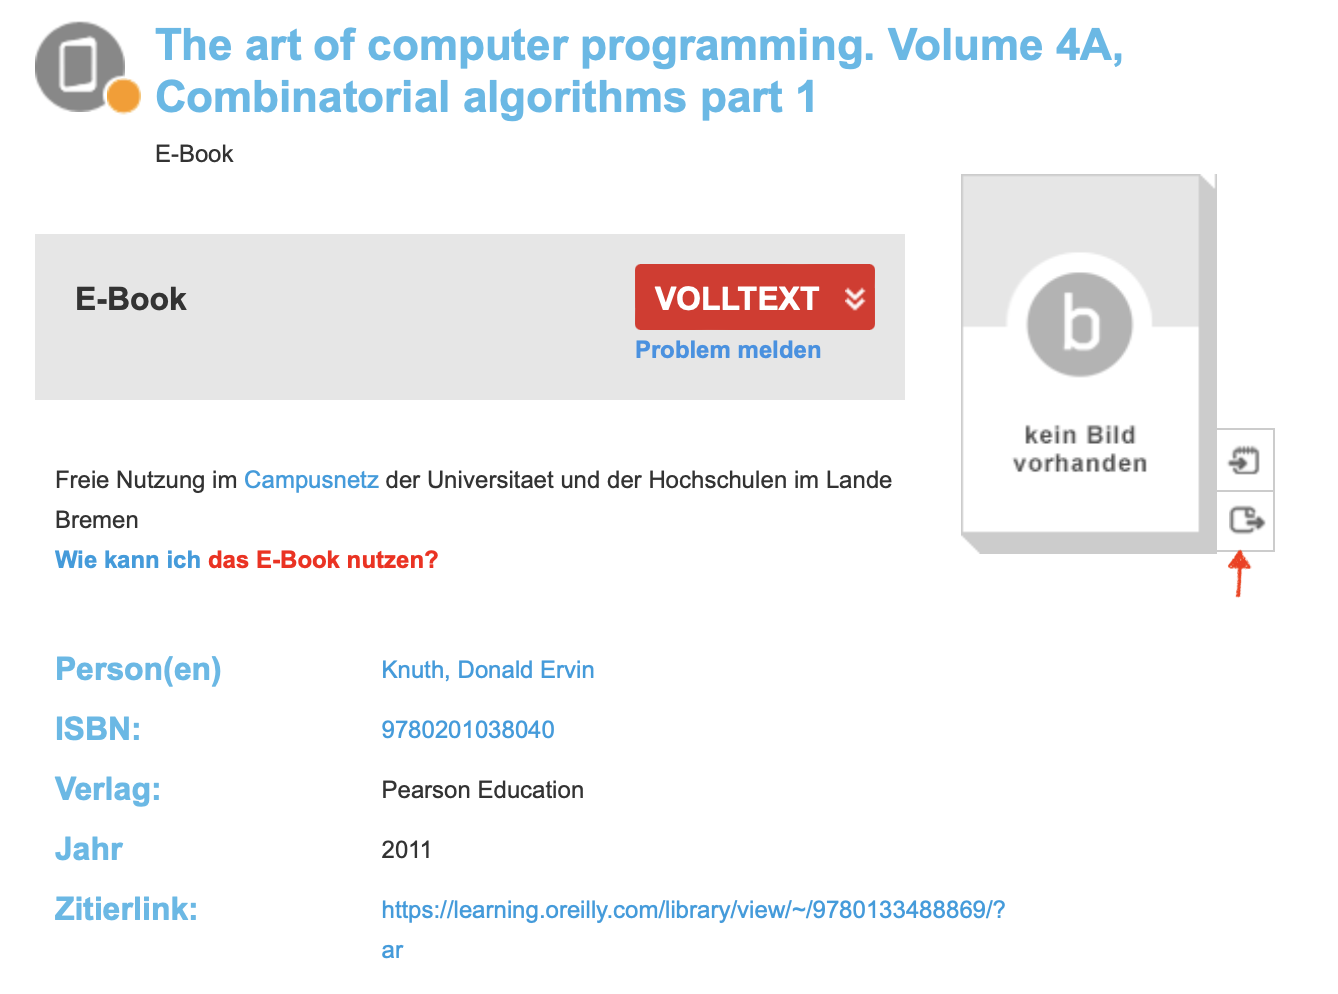
\includegraphics[width=0.65\textwidth]{src/abbildungen/export.png}
	\caption{BibTeX Einträge exportieren}
\end{figure}
\FloatBarrier

Die Möglichkeit sich zu Artikeln, Büchern, Sammelbänden etc. die passenden
BibTeX Einträge generieren zu lassen, wird auf den entsprechenden Seiten quasi
flächendeckend angeboten. Resultat eines solchen Exports ist ein einzelner
BibTeX Eintrag, dieser kann dann in der \texttt{hauptdatei.bib} hinterlegt
werden. 

\FloatBarrier
\begin{figure}[ht!]
	\centering
	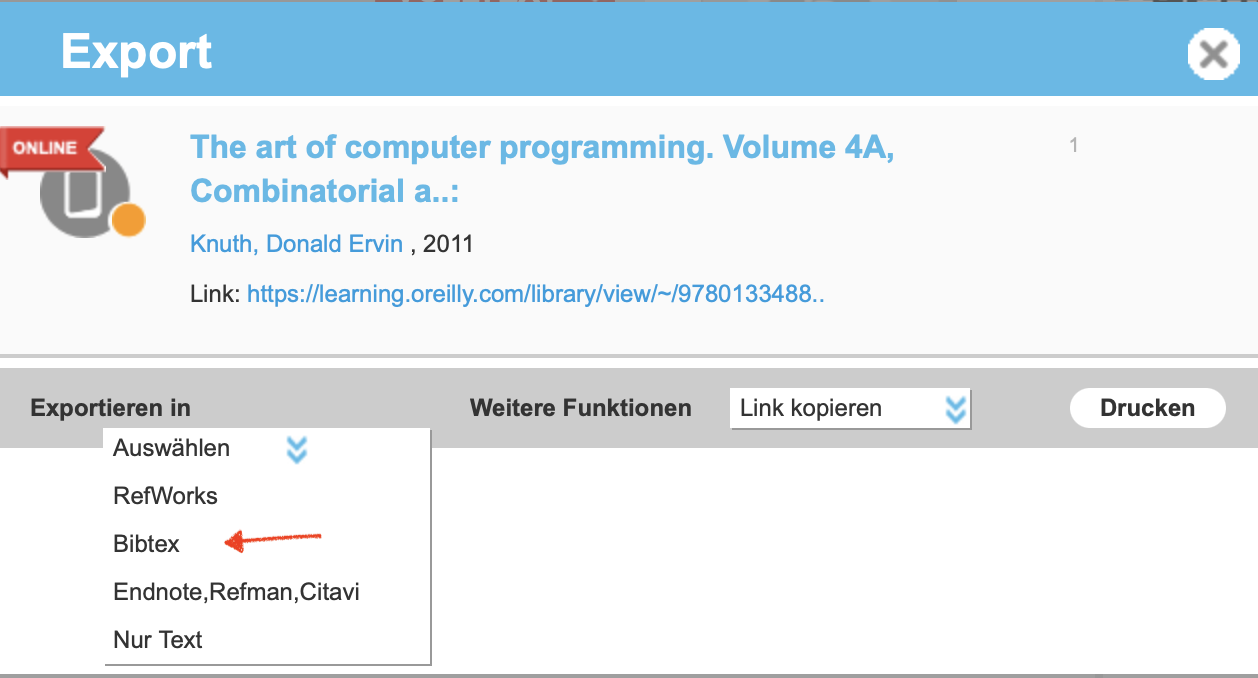
\includegraphics[width=0.65\textwidth]{src/abbildungen/bibtex.png}
	\caption{BibTeX Einträge exportieren (Formatauswahl)}
\end{figure}
\FloatBarrier

\begin{code}{Beispiel BibTeX Eintrag}{beispielbibtex}
	\begin{minted}{latex}
		@book{Thea2011,
		title = {The art of computer programming. Volume 4A, Combinatorial algorithms part 1},
		author = {Donald Ervin Knuth},
		publisher = {Pearson Education},
		year = {2011},
		note = {1 volume},
		ISBN = {9780201038040},
		URL = {https://learning.oreilly.com/library/view/~/9780133488869/?ar},
		}
	\end{minted}
\end{code}

Im Laufe einer Hausarbeit wird unsere persönliche Bibliothek eine Vielzahl
solcher Einträge enthalten. Die Einträge enthalten jeweils einen Typ, im obigen
Beispiel \texttt{book} und ein Kürzel, in diesem Fall \texttt{Thea2011}. Es 
existieren viele verschiedene Typen von Einträgen, in den meisten Fällen werden
wir unsere Einträge, wie gezeigt, exportieren können, es ist natürlich auch
möglich, eigene Einträge zu erstellen. Hauptsächlich tue ich dies, wenn es sich
um Webseiten oder ähnliche Onlinequellen handelt. 
Ein solcher Eintrag lässt sich gemäß nachstehendem Format erstellen: 

\begin{code}{Beispiel BibTeX Eintrag (Onlinequelle)}{beispielbibtexonline}
	\begin{minted}{latex}
		@online{flignitz,
		title = {How-to LaTeX},
		url = {https://informatik.hs-bremerhaven.de/flignitz/latex.html},
		urldate = {2023-04-18},
		Author = {Fabian Lignitz},
		Language = {de},
		Month = {04},
		Year = {2023},
	  }
	\end{minted}
\end{code}

Soll eine Literaturangabe nach einem Zitat oder Paraphrase angefügt werden, ist
dies durch das Kommando \texttt{\textasciitilde\textbackslash autocite[]\{\}}
möglich. Zur Veranschaulichung sollen uns einige kleine Beispiele dienen: 

\glqq In general, each prime implicant corresponds in this way to a maximal
subcube that stays within the set of points that make f
true~\autocite[]{KnutThea2009}.\grqq{}

\begin{quote}
	\footnotesize{	
	When you hear about this problem for the first time, you might be tempted
	to ask a question of your own in return: \glqq What? Are you serious that computer
	scientists still haven’t figured out how to do such a simple
	thing?\grqq{}~\autocite[S.432]{KnutThea2009}
	}
\end{quote}

Gemäß Lignitz~\autocite[]{flignitz} biete BibLaTeX einen besseren Umgang mit
Umlauten und Onlinequellen, als dies mit BibTeX möglich wäre.

Wie in den Beispielen zu sehen, kann an jeder beliebigen Stelle zitiert werden,
zusätzlich kann in den eckigen Klammern eine Seitenzahl angegeben werden, dies
ist jedoch nicht nötig. Zu beachten gilt, dass eingerückte Zitate keine
Anführungsstriche erhalten, jedoch in diesem Fall in der Quelle
Anführungsstriche gesetzt wurden und diese beibehalten werden müssen. Paraphrasen 
erhalten in keinem Fall Anführungszeichen. In \LaTeX~sehen die Beispiele wie folgt aus: 

\begin{code}{Beispiele zitieren}{beispielzitate}
	\begin{minted}{latex}
		\glqq In general, each prime implicant corresponds in this way to a maximal
		subcube that stays within the set of points that make f
		true~\autocite[]{KnutThea2009}.\grqq{}
		
		\begin{quote}
			\footnotesize{	
			When you hear about this problem for the first time, you might be tempted
			to ask a question of your own in return: \glqq What? Are you serious that computer
			scientists still haven’t figured out how to do such a simple
			thing?\grqq{}~\autocite[S.432]{KnutThea2009}
			}
		\end{quote}
		
		Gemäß Lignitz~\autocite[]{flignitz} biete BibLaTeX einen besseren Umgang mit
		Umlauten und Onlinequellen, als dies mit BibTeX möglich wäre.	
	\end{minted}
\end{code}

Sobald wir in unserem Fließtext zitieren, wird entsprechend des gewählten
Zitierstils auch das Literaturverzeichnis gebaut. Dies findet ihr am Ende des
Hauptteils als erstes Verzeichnis. Durch die Verwendung von BibTeX brauchen wir 
uns also weder um das Anlegen von Literaturverzeichnis, noch um die Nummerierung
oder Reihenfolge von Literaturangaben zu kümmern. Es reicht lediglich mittels des 
\texttt{\textasciitilde\textbackslash autocite[]\{\}} Kommandos und des richtigen
Kürzels im Fließtext eine Literaturangabe zu setzen. 

